\section{Introduction} \label{sec:intro}
\subsection{Background}

Our accelerating computational demand and the rise of multicore hardware
have made multithreaded programs pervasive and critical.  Yet,
these programs remain extremely difficult to write, test, analyze, debug,
and verify.  A key reason is that, for decades, the contract between
developers and thread runtimes has favored performance over
correctness.  In this contract, developers use 
synchronizations to coordinate threads, while thread runtimes can
use \emph{any} of the exponentially many thread interleavings, or \emph{schedules}, compliant
with the synchronizations.  This large number of possible schedules make it
more likely to find an efficient schedule for a workload, but ensuring
that all schedules are free of concurrency bugs is extremely
challenging, and a single missed schedule may surface in the least
expected moment, causing critical
failures~\cite{therac25-investigation, northeast-blackout,
  lu:concurrency-bugs,con:hotpar12}.
%%  This contract harms a critical 
%% property, \emph{repeatability}, that developers anticipate, that is, 
%% similar inputs should lead to similar behaviors from runs to runs.

%% For decades, the contract between developers and thread runtimes has been
%% that developers puts synchronizations in code to prevent all buggy thread
%% schedules, while the runtimes are free to use \emph{any} of all schedules
%% compliant with the synchronizations.

%% For instance, $n$
%% threads competing for a lock easily yields $n!$ schedules because the
%% threads may arrive at the lock operations in $n!$ orders.

%% In order to achieve repeatabilty for multithreaded programs 
%% on the same input, 
Several recent systems aim to flip this performance vs correctness tradeoff
by reducing the number of allowed schedules.  Among them,
\emph{deterministic multithreading} (DMT)
systems~\cite{coredet:asplos10,dmp:asplos09, kendo:asplos09,
  grace:oopsla09, cui:tern:osdi10, dthreads:sosp11, determinator:osdi10,
  peregrine:sosp11, bergan:oopsla13} reduce schedules by mapping each input to only one
schedule, so that executions of the same program on the same input always
show the same behavior. DMT is commonly believed to simplify testing,
debugging, record-replay, and replication of multithreaded programs.

However, we argue that determinism is not as useful as commonly perceived:
it is neither sufficient nor necessary for
reliability~\cite{smt:hotpar13,smt:cacm}.  It is not sufficient because it
is quite narrow (``same input + same program = same behavior'') and has no
jurisdiction if the input or program changes however slightly.  For
instance, a perfectly deterministic system can map each input to an
arbitrary schedule, so that flipping
an input bit or adding a line of debug code leads to vastly different schedules,
artificially reducing the program's robustness against input and program
perturbations, or \emph{stability}.  Yet stability is crucial
for reliability (\eg, after testing some inputs, developers often anticipate that the program work on many similar inputs). Determinism is not necessary for
reliability because a nondeterministic system with a small set of
schedules for all inputs can be made reliable by exhaustively checking all
schedules.

%% Unfortunately, the repeatability of determinized execution is subject to
%% changing inputs,
%% %% Unfortunately, determinism is only a narrow repeatability concerning each
%% %% individual input, 
%% and some DMT systems actually harm other aspects of
%% repeatability developers anticipate, such as ``similar inputs lead to
%% similar behaviors'' and ``adding debug \v{printf} doesn't mask bugs.''  The
%% reason is that these systems process each input with an arbitrary
%% schedule~\cite{coredet:asplos10, kendo:asplos09}, so slight input or
%% program changes may lead to drastically different schedules, destabilizing
%% program behaviors~\cite{cui:tern:osdi10}.  Moreover, the total set of
%% schedules for all inputs remains enormous, still demanding practically
%% infinite resources to check.

%\footnote{We borrowed the term from~\cite{smt-tr}.}

%% We believe that what makes multithreading challenging is quantitative:
%% multithreaded programs have \emph{too many} schedules.  The number of
%% schedules for each input is already enormous because the parallel threads
%% may interleave in many ways, depending on such factors as hardware timing
%% and operating system scheduling.  Aggregated over all inputs, the number
%% is even greater.  Finding a few buggy schedules out of an enormous number
%% of schedules (so developers can prevent them) is like finding a few
%% needles in a haystack.  Although DMT reduces schedules for each input, it
%% may map each input to a different schedule, so the total set of schedules
%% for all inputs remains vast.


We propose a better approach we call \emph{stable multithreading
  (\smt)}~\cite{smt:cacm,smt:hotpar13} that reuses each schedule on a wide
range of inputs, mapping all inputs to a dramatically reduced set of
schedules.  For instance, under most setups, \smt reduces the number of
schedules needed by parallel compression utility \pbzip down to \emph{two}
schedules for each different number of threads, regardless of the file
contents~\cite{peregrine:sosp11}.  By vastly shrinking the set of schedules, \smt makes it
extremely easy to find the schedules that cause concurrency bugs.  Specifically,
\smt greatly increases the coverage of tools that
systematically test schedules for
bugs~\cite{musuvathi:chess:osdi08,modist:nsdi09,godefroid:verisoft,dbug:spin11}.
It also greatly improves the precision and simplicity of program
analysis~\cite{wu:pldi12}, verification~\cite{wu:pldi12}, and debugging,
which can now focus on a much smaller set of schedules.  Moreover, \smt
makes programs robust against small input or program perturbations,
bringing stability into multithreading.

\smt is not mutually exclusive with DMT.  \grace~\cite{grace:oopsla09},
\tern~\cite{cui:tern:osdi10}, \determinator~\cite{determinator:osdi10},
\peregrine~\cite{peregrine:sosp11}, and \dthreads~\cite{dthreads:sosp11}
may all be classified as both deterministic and stable. Prior
work~\cite{dthreads:sosp11,cui:tern:osdi10,peregrine:sosp11,determinator:osdi10},
including ours~\cite{cui:tern:osdi10,peregrine:sosp11}, conflated
determinism and stability, but they are actually separate properties.

% To reproduce a buggy schedule for debugging, developers need consider a
% much smaller set of schedules.

\begin{figure*}[t]
\begin{center}
\subfloat[{\em Traditional.}]{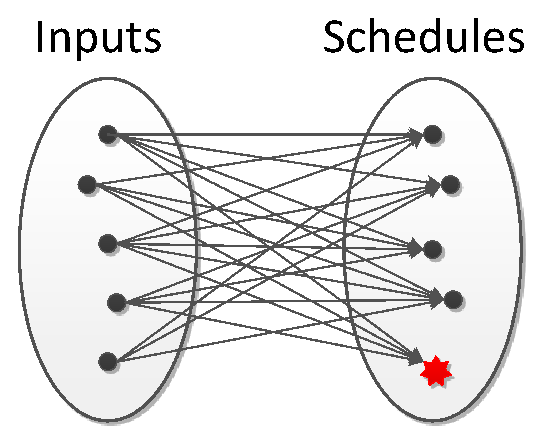
\includegraphics[width=.20\linewidth]{figures/nondet}\label{fig:nondet}}
\subfloat[{\em Deterministic.}]{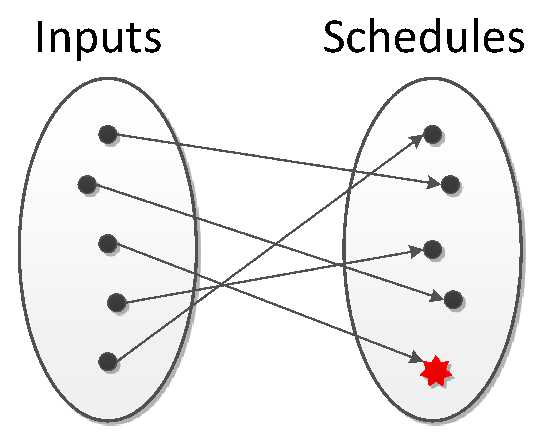
\includegraphics[width=.20\linewidth]{figures/dmt}\label{fig:dmt}}
\subfloat[{\em Stable (deterministic).}]{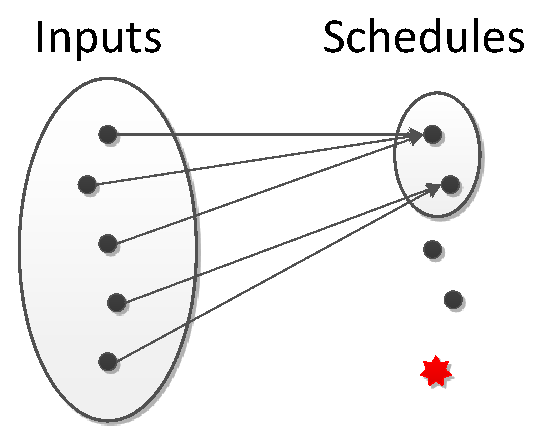
\includegraphics[width=.20\linewidth]{figures/smt}\label{fig:smt}}
\subfloat[{\em Stable (nondeterministic).}]{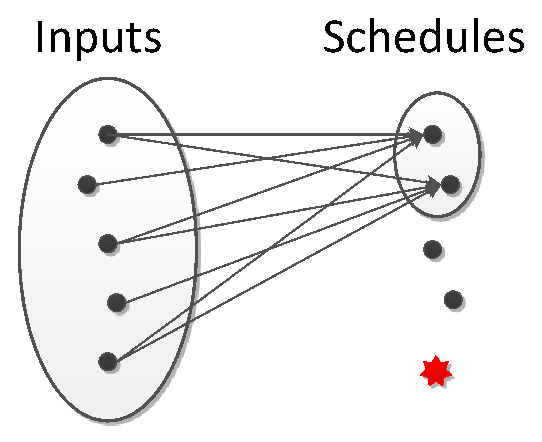
\includegraphics[width=.20\linewidth]{figures/smtn}\label{fig:smtn}}
\vspace{-.05in}
\caption{{\em Different multithreading approaches.} Stars in red represent
  schedules that cause concurrency bugs.} \label{fig:mt}
\vspace{-.2in}
\end{center}
\end{figure*}

Figure~\ref{fig:mt} compares traditional multithreading, DMT, and \smt.
Figure~\ref{fig:nondet} depicts traditional multithreading, a conceptual
many-to-many mapping between inputs and schedules.  Figure~\ref{fig:dmt}
depicts a DMT system that maps each input to an arbitrary schedule,
artificially destabilizing program behaviors.  Figures~\ref{fig:smt}
and~\ref{fig:smtn} depict two \smt systems: the many-to-one mapping in
Figure~\ref{fig:smt} is deterministic, while the many-to-few mapping in
Figure~\ref{fig:smtn} is nondeterministic.  A many-to-few mapping improves
performance by giving the runtime choices, but it
increases the checking effort needed for reliability.  Fortunately, the
choice of schedules is minimal, so that tools can easily achieve
high coverage.

%% To solve these issues, several \emph{stable multithreading}
%% (\smt)~\cite{smt-tr} systems~\cite{cui:tern:osdi10, grace:oopsla09,
%%   dthreads:sosp11, determinator:osdi10, peregrine:sosp11} reduce the total
%% set of schedules for all inputs.  They enforce well-defined
%% synchronization schedules, each of which
%% can be reused on a wide range of inputs and slightly modified programs,
%% providing much broader repeatability than just determinism.  For
%% instance, given the same thread count and file block count, the parallel
%% compression utility \pbzip~\cite{pbzip2} can use the same schedule to compress any file,
%% regardless of file data.  By vastly reducing the number of schedules
%% needed, \smt also greatly increases testing coverage defined as the ratio
%% of tested schedules over all schedules.  Moreover, \smt greatly simplifies
%% static analysis and verification because these approaches can now focus
%% only on the small set of \smt-enforced schedules~\cite{wu:pldi12,smt-tr}.
%% \smt is not mutually exclusive with DMT.  \grace~\cite{grace:oopsla09},
%% \tern~\cite{cui:tern:osdi10}, \determinator~\cite{determinator:osdi10},
%% \peregrine~\cite{peregrine:sosp11}, and \dthreads~\cite{dthreads:sosp11}
%% may all be classified as both deterministic and stable.


%% In contrast, \emph{stable multithreading} (\smt)
%% systems~\cite{cui:tern:osdi10,peregrine:sosp11,smt-tr} reduce the set of
%% schedules for all inputs by reusing the same schedules on similar inputs
%% or even slightly modified programs.  For instance, they reduced the
%% schedules for parallel compression utility \pbzip to compress \emph{any}
%% file down to two schedules per thread count.  \smt provides much broader
%% repeatability and, by shrinking the ``haystack,'' greatly simplifies
%% checking schedules.  \smt systems can be deterministic.  For instance,
%% \peregrine~\cite{peregrine:sosp11}, \dthreads~\cite{dthreads:sosp11}, and
%% \determinator~\cite{determinator:osdi10} may all be classified as both
%% stable and deterministic.  \smt systems can also be nondeterministic, as
%% long as the number of schedules for an input is small so the problems
%% caused by nondeterminism are easy to solve.  For instance, to reproduce a
%% bug, developers easily afford to run the program a few times.
%% \tern~\cite{cui:tern:osdi10} is an example \smt system that provides only
%% best-effort determinism for programs that contain data races.

%% Although researchers have shown promising results on a small number of
%% programs, it remains an open question whether the DMT or \smt approach has
%% any hope of being practical.  A main concern is whether the approaches can
%% consistently achieve good performance on many programs.  Schedules should
%% be oblivious to local computations for repeatability and checking
%% coverage, yet they must also handle the computations efficiently.  It is
%% extremely challenging to reconcile these two conflicting goals, so prior
%% systems required a variety of heavyweight techniques and unrealistic
%% assumptions (cf \S\ref{sec:related}). As usual, it takes years, if not
%% forever, to adopt heavyweight techniques (\eg, new
%% hardware~\cite{dmp:asplos09}, new languages~\cite{dpj:oopsla09}, new
%% programming models~\cite{determinator:osdi10}, costly execution
%% recording~\cite{cui:tern:osdi10, peregrine:sosp11}, or sophisticated
%% program analysis~\cite{coredet:asplos10,peregrine:sosp11}).  Unrealistic
%% assumptions severely limit applicability (\eg, only fork-join
%% parallelism~\cite{grace:oopsla09}) or incur large overhead on many
%% programs (\eg, schedules serialize all intended parallel computations; see
%% \S\ref{sec:example} and \S\ref{sec:comparison}).

%% It is extremely challenging to reconcile the conflicting goals of making
%% schedules (1) oblivious to computations to maximize repeatability and
%% checking coverage and (2) efficient to carry out the computations
%% developers intend.  Yet, prior systems cut developers out of the loop when
%% solving this challenge, and required a variety of heavyweight techniques
%% and unrealistic assumptions for performance.  As usual, heavyweight
%% techniques---\eg, new hardware~\cite{dmp:asplos09}, new
%% languages~\cite{dpj:oopsla09}, new programming
%% models~\cite{determinator:osdi10}, or costly execution
%% recording~\cite{cui:tern:osdi10, peregrine:sosp11}, and sophisticated
%% program analysis~\cite{coredet:asplos10,peregrine:sosp11})---take years,
%% if not forever, to adopt. Systems with unrealistic assumptions---\eg, only
%% fork-join parallelism~\cite{grace:oopsla09} or computation-oblivious
%% schedules magically align with
%% computations~\cite{dthreads:sosp11}---either cannot support many
%% real-world programs or deterministically slow them down to the extent that
%% intended parallel computations are pathologically serialized (cf
%% \S\ref{sec:} for an example and \S\ref{sec:eval} for performance results).

%% Worse, because of the deterministic nature of prior systems, developers
%% are stuck with the inefficient schedules.

%% By eliminating many
%% schedules, prior systems potentially gain reliability, but they sometimes
%% severely harm performance if the chosen schedules cannot react well to the
%% workloads.

%% Unfortunately, they do so by providing a unilateral, inflexible contract
%% that cuts developers out of the loop:

%% Although researchers have shown promising results on a small number of
%% programs, it remains an open question whether DMT or \smt has any hope of
%% being practical.  A main concern is performance.  A runtime with much
%% fewer schedules in principle gains reliability, but it may severely hurt
%% performance if a given workload and the selected schedule mismatch.  Yet,
%% without knowing how developers intend to process a workload in parallel,
%% it is extremely challenging to reconcile the two conflicting goals of (1)
%% vastly reducing schedules and (2) selecting a reasonably efficient
%% schedule.  Prior systems cut developers out of the loop when solving this
%% challenge, and thus have to employ a variety of heavyweight techniques and
%% impractical restrictions for performance.  Some require new hardware,
%% programming languages, or programming models~\cite{xxx}, which take years,
%% if not forever, to adopt.  Some approximate actual execution time by
%% counting instructions each thread executes, but a small input or program
%% change may lead to much different schedules, destabilizing program
%% behaviors~\cite{xxx}.  Some require heavyweight recording and
%% sophisticated program analysis~\cite{xxx}.  Some require that \emph{all}
%% threads in a program do synchronizations at roughly the same rate, and our
%% experiments show that they incur up to XXX overhead on programs not
%% meeting this unrealistic requirement by serializing parallel computations
%% (\S\ref{sec:eval}).

%% A second concern is whether the approaches can handle the diverse
%% constructs real-world programs depend upon.  Our experiments show that two
%% prior systems~\cite{coredet:asplos10, dthreads:sosp11} lack support for
%% many of these constructs, and failed on XXX out of XXX programs
%% (\S\ref{sec:eval}).  While some unsupported constructs such as POSIX
%% semaphores may be added without too much double, other constructs
%% especially network operations (\eg, \v{send} and \v{recv}) and
%% nondeterministic timeout operations (\v{sleep} and \pthread \v{timedwait}
%% functions) are much more challenging.  Not or na\"{i}vely supporting them
%% lead to huge performance overhead and even deadlocks (\S\ref{sec:eval}).

%% A third concern is whether the approaches can effectively improve
%% reliability.  Although in theory they do, in practice almost no
%% quantitative studies have demonstrated so, and researchers have argued
%% that some DMT systems may harm reliability.  In fact, to our knowledge, no
%% studies at all have shown that the approaches benefit testing tools,
%% making it difficult to evaluate the performance and reliability tradeoff.
%% Consider \emph{model checkers} that systematically test different orders
%% of nondeterministic events such as synchronizations and network I/Os for
%% bugs~\cite{modist:nsdi09, dbug:spin11, yang:explode:osdi, yang:fisc:osdi,
%%   killian:macemc:nsdi07, demeter:sosp11}. They can enjoy greatly improved
%% coverage by greatly reducing schedules.  Yet, how can we integrate a model
%% checker with a DMT or \smt system?  Both must control the order of
%% nondeterministic events, and may run into deadlocks if they interfere with
%% each other.

%None of these concerns is helped much by the fact that (1) prior work has

\subsection{Challenges}

Although the latest advances are promising, two important challenges remain
unaddressed.  First, can the DMT and \smt approaches consistently achieve
good performance on a wide range of programs?  For instance, we observed
that a prior system, \dthreads, had 5$\times$ to 100$\times$ slowdown on
some programs.  Second, can they be made simple and adoptable?
These challenges are not helped much by the limited
evaluation of prior systems which often used (1) synthetic benchmarks, not
real-world programs, from incomplete benchmark suites; (2) one workload
per program; and (3) at most 8 cores (with three exceptions; see \S\ref{sec:related}).

These challenges are intermingled.  Reducing schedules improves correctness
but trades performance because the schedules left may not balance each
thread's load well, causing some threads to idle unnecessarily.  Our
experiments show that ignoring load imbalance as in \dthreads
can lead to pathological
slowdown if the order of operations enforced by a schedule
\emph{serializes} the intended parallel computations
(\S\ref{sec:comparison}).  To recover performance, one method is to count
the instructions executed by each thread and select schedules that balance
the instruction counts~\cite{kendo:asplos09, coredet:asplos10,
  dmp:asplos09}, but this method is not stable because input or program
perturbations easily change the instruction counts.  The other method (we proposed)
lets the nondeterministic OS scheduler select
a reasonably fast schedule and reuses the schedule on
compatible inputs~\cite{cui:tern:osdi10,peregrine:sosp11}, but it
requires sophisticated program analysis, complicating deployment.

%% This performance concern is not much helped by the limited evaluation of
%% prior systems.  First, prior work has reported results on only a narrow
%% set of programs, typically less than 15.  The programs are almost always
%% synthetic benchmarks, not real-world programs.  No results on any complete
%% benchmark suite has been reported, and the handpicked benchmarks are
%% usually simpler and have lower overhead than the ones left out.  Second,
%% the experimental setups are limited, often with one unspecified or
%% handpicked workload per program and up to 8 cores when standard
%% servers have several times more cores.  Lastly, prior work generally has
%% not demonstrated how the approaches benefit testing or reported any
%% quantitative results on improving correctness, making it difficult for
%% potential adopters to justify the overhead.

%% Unsurprisingly, two prior
%% systems~\cite{coredet:asplos10,dthreads:sosp11} we tried failed on XXX of
%% the \nprog programs we evaluated and cannot support many constructs
%% real-world programs depend upon, including network operations (\eg,
%% \v{send} and \v{recv}) and nondeterministic timeout operations (\v{sleep}
%% and \pthread \v{timedwait} functions).

%; and (4) results of only up to 8 cores were reported, while typical
%; servers now have three times many cores.

\subsection{Contributions}

This paper makes three contributions.
%% YJF: DON'T move \footnote before comma. check grammar
First, we present \xxx,\footnote{We name our system after one of the most
  trainable birds.} a simple, practical runtime that efficiently makes
threads deterministic and stable by offering a new contract to developers.
By default, it schedules synchronizations in each thread using
round-robin, vastly reducing schedules and providing broad repeatability.
When default schedules are slow, it allows advanced developers to add
intuitive \emph{performance hints} to their code for speed.  Developers discover
where to add hints through profiling as usual, and \xxx simplifies
performance debugging by deterministically reproducing the bottlenecks.
The hints are robust to developer mistakes as they can be safely ignored
without affecting correctness.

Like prior systems, \xxx's contract reduces schedules to favor correctness over performance.  Unlike prior systems, it allows advanced developers
to optimize performance.  We believe this practical ``meet in the
middle'' contract eases writing correct, efficient programs.

% based on several years of lessons.

%% Like prior systems, \xxx's contract favors correctness over performance
%% by vastly reducing schedules.  Unlike prior systems, it provides
%% advanced developers the flexibility for better performance.

\xxx provides two performance hint abstractions.  A \emph{soft
  barrier} encourages the scheduler to coschedule a group of threads at
given program points.  It is for performance only, and operates as a
barrier with deterministic timeouts in \xxx.  Developers use it to switch
to faster schedules without compromising determinism
when the default schedules serialize parallel
computations (\S\ref{sec:example}).  A \emph{performance critical section}
informs the scheduler that a code region is a potential
bottleneck, encouraging the scheduler to get through the region fast.
When a thread enters a performance critical section, \xxx delegates scheduling to the
nondeterministic OS scheduler for speed.  
Performance critical sections may trade some determinism for
performance, so they should be applied only when the schedules they add
are thoroughly checked by tools or advanced developers.
These simple abstractions
let \xxx run fast on all programs evaluated, and
may benefit other DMT or \smt systems and classic nondeterministic
schedulers~\cite{coschedule:sigmetrics96, coschedule, partial-barrier:atc06}.

%% \xxx currently supports two types of performance hints.  \emph{Computation
%%   hints} inform \xxx of a group of computations developers intend to run
%% in parallel, so \xxx can switch to faster schedules.  \emph{Nondeterminism
%%   hints} inform \xxx of carefully chosen code regions developers intend to
%% revert back to nondeterminism execution for, so \xxx can use the
%% additional schedules for performance.  Mixing deterministic and
%% nondeterministic executions is tricky because they may interfere; we have
%% carefully defined the semantics of the nondeterminism hints to provably
%% avoid interference (\S\ref{sec:hints}).  These simple hints let \xxx
%% achieve low overhead on all \nprog programs evaluated while avoiding
%% heavyweight techniques and unrealistic assumptions.  They can also benefit
%% other DMT or \smt systems and even nondeterministico thread runtimes.

Our \xxx implementation is \pthread-compatible, simplifying deployment.
It handles many diverse constructs real-world programs depend upon such as
network operations and timeouts.  \xxx makes synchronizations outside
performance critical sections deterministic but allows nondeterministic
data races.  Although it is
straightforward to make data races deterministic in \xxx,
% with a memory commit protocol we designed, 
we deemed it not worthwhile because the cost of doing so outweighs the
benefits (\S\ref{sec:discussion}).  \xxx's determinism is similar to
\kendo's weak determinism~\cite{kendo:asplos09}, but \xxx offers stability
which Kendo lacks.

%% \xxx currently is not intended to make data races deterministic.  Although
%% doing so is straightforward (cf \S\ref{sec:xxx} for a memory commit
%% protocol we designed to let \xxx make data races deterministic), we deem
%% it not worthwhile.  Prior work~\cite{peregrine:sosp11,pres:sosp09} has
%% shown that data races rarely occur if a synchronization schedule is
%% enforced (\eg, xxx data races out of xxx millions of memory accesses).
%% The occurred races are often benign ad hoc
%% synchronizations~\cite{syncfinder:osdi10} that require developer
%% annotations anyway~\cite{dthreads:sosp11}.  The remaining races are so
%% rare that it is possible to detect or reproduce them by searching through
%% a small number of executions~\cite{pres:sosp09} using for example model
%% checkers.

Our second contribution is an ecosystem formed by integrating \xxx with
\dbug~\cite{dbug:spin11}, an open source model checker for 
distributed and multithreaded Linux programs that systematically checks possible schedules for bugs.
This \ecosys ecosystem is more effective than
either system alone: \dbug checks the schedules
that matter to \xxx and developers (\eg, schedules added by performance
critical sections), and \xxx greatly increases \dbug's coverage by
reducing the schedules \dbug has to check (the \emph{state space}). Our
integration is transparent to \dbug and requires only minor
changes to \xxx.  It lets \xxx effectively leverage advanced model
checking techniques~\cite{flanagan:dynamicpo, demeter:sosp11}.
%, such as effective search heuristics and reduction
% techniques~\cite{flanagan:dynamicpo} which soundly avoid checking
% equivalent executions.

%% that we quantitatively show that \xxx
%% effectively improves correctness by integrating \xxx with \dbug, a model
%% checker that systematically tests different orders of nondeterministic
%% events for bugs.  This integration is mutually beneficial: \xxx greatly
%% increases \dbug's coverage by vastly reducing schedules, and \dbug checks
%% the schedules that matter to \xxx, including the default schedules,
%% schedules selected by \compute, and schedules added by \nondet.

%% Both \xxx and \dbug must control the order of nondeterministic events, and
%% may run into deadlocks if they interfere with each other.  To solve this
%% challenge, our \xxx and \dbug integration uses a nested scheduler
%% architecture with \xxx nesting inside \dbug.  \xxx deterministically
%% schedules synchronizations, and exposes only synchronizations in \nondet
%% regions to \dbug.  \dbug then systematically explores the order of these
%% synchronizations and other nondeterministic events such as network
%% operations.  This architecture makes the integration seamless, and
%% required only XXX lines of modification to \xxx and zero to \dbug.  It
%% illustrates an additional \smt advantage: \xxx enforces the same
%% well-defined schedules whether it runs alone or inside \dbug.

Third, we quantitatively show that \xxx achieves good performance and high
model checking coverage on a diverse set of \nprog programs.  The programs
include \nrealprog real-world programs, such as \bdb~\cite{berkeleydb},
\openldap~\cite{openldap}, \redis~\cite{redis}, \mplayer~\cite{mplayer},
all \nstl parallel C++ STL algorithm 
implementations~\cite{parallel-stl} which use \openmp, and all \nimagick
parallel image processing utilities (also \openmp) in the \imagick~\cite{imagick}
software suite.  Further, they
include \emph{all} \nbenchmarks programs in four widely used benchmark suites:
\parsec~\cite{parsec}, \phoenix~\cite{phoenix-benchmarks}, \splashx~\cite{splashx},
and \npb~\cite{npb}.  We used complete software or benchmark suites to
avoid biasing our results. The programs together cover many different
parallel programming models and idioms such as threads,
\openmp~\cite{openmp}, fork-join, map-reduce, pipeline, and workpile.  To
our knowledge, our
evaluation uses roughly \overeach more programs than any prior
DMT or \smt evaluation, and \overcombined more than all
prior evaluations combined.
% We used at least three different scales/types of workloads per program
% and a 24-core machine to make our results robust.
Our experiments show:
\begin{tightenum}

\item \xxx is easy to use. It averages only \hintsperprog lines of hints
  per program to get good performance, and adding hints is fast.  Of all
  \nprog programs, \nprognohints need no hints, \nproglineuphints need
  \computes which do not affect determinism, and only \nprognondethints
  programs need \nondets to trade some determinism for speed.

\item \xxx has low overhead.  At the maximum allowed (16--24) cores, \xxx's
  geometric mean overhead is \meanrealoverhead for \nrealprog real-world programs,
  \meanbenchoverhead for the other \nbenchmarks programs, and \meanoverhead for all.

\item On \nprogcompared programs that two prior systems \dthreads~\cite{dthreads:sosp11}
  and \coredet~\cite{coredet:asplos10} can both handle, \xxx's overhead is \xxxcompoverhead whereas \dthreads's
  is \dthreadssyncoverhead and \coredet's \coredetoverhead.

\item \xxx scales well to the maximum allowed cores on our 24-core server and
  to at least three different scales/types of workloads per program.

\item \ecosys offers exponential coverage increase compared to \dbug alone.
  \xxx helps \dbug reduce the state space by \shrinkscale for
  \nprogshrink programs and increase the number of verified programs from
  \nprogverifieddbug to \nprogverifiedxxx under our test setups.
  These verified programs include all 4 real-world programs out of
  the \nprognondethints programs that need performance critical sections, so they
  enjoy both speed and reliability.
  These quantitative reliability results help potential \xxx adopters justify
  the overhead.

\end{tightenum}

We have released \xxx's source code, entire benchmark suite, and
raw results~\cite{Parrot:github}. In the remaining of this paper, $\S$\ref{sec:overview} contrasts \xxx with 
prior systems on an example and gives an overview of \xxx's 
architecture.~$\S$\ref{sec:hints} describes the performance hint abstractions \xxx
provides,~$\S$\ref{sec:runtime} the \xxx runtime, and~$\S$\ref{sec:mc} the
\xxx-\dbug ecosystem.~$\S$\ref{sec:discussion} discusses \xxx's determinism,~$\S$\ref{sec:eval}
presents evaluation results,~$\S$\ref{sec:related}
discusses related work, and~$\S$\ref{sec:conclusion} concludes.
